%!TEX root = chi14grammatical.tex
\begin{figure*}[th]
\begin{subfigure} {1.4\columnwidth}
			\centering
	\fbox{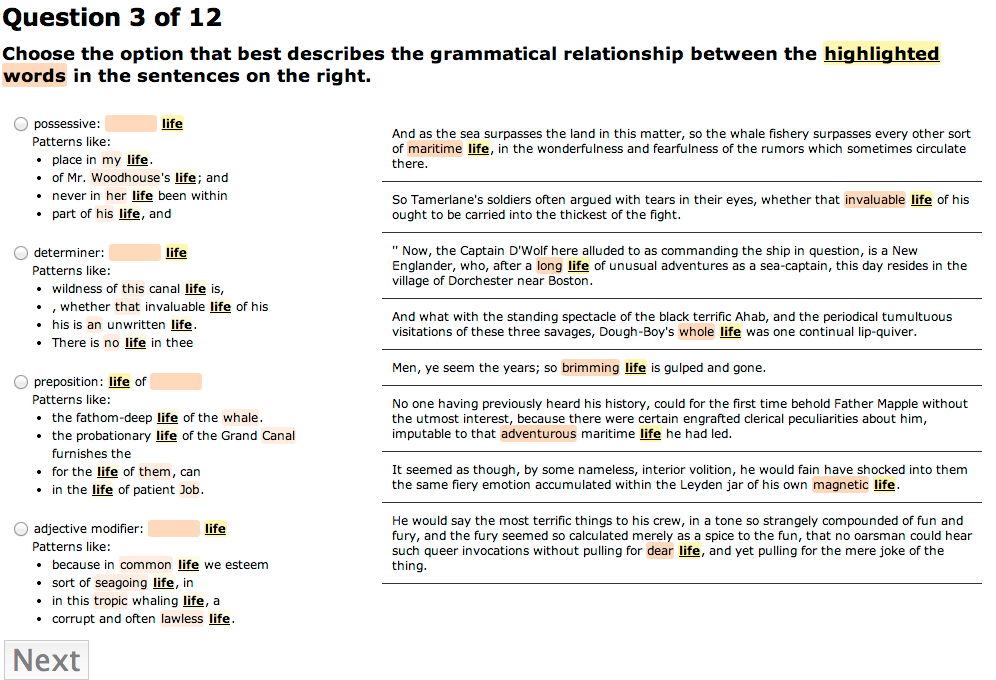
\includegraphics[width=\columnwidth]{fig/task}}
	\caption{\label{fig:task} An example of an identification task in the \emph{phrases} condition for the relationship \code{amod(life, \_\_\_)} (where different adjectives modify the noun `life'). The correct answer is `adjective modifier' (4th option), and the remaining 3 options are distractors.}
	\end{subfigure}
	\qquad
	\begin{subfigure}{0.7\columnwidth}
		\begin{subfigure}{0.7\columnwidth}
				\centering
		\fbox{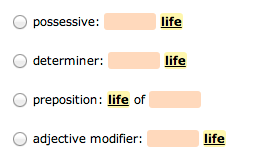
\includegraphics[width=\columnwidth]{fig/baseline-choices}}
	    \caption {The same options as they appear in the \emph{baseline} condition. \label{fig:baseline-choices}}
	    \end{subfigure}

	    \begin{subfigure}{0.7\columnwidth}
	    	\centering
	    	\fbox{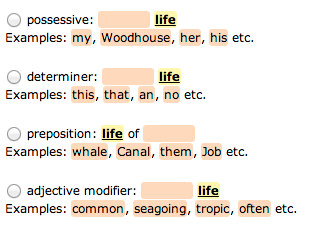
\includegraphics[width=\columnwidth]{fig/words-choices}}
	        \caption {The same options as they appear in the \emph{words} condition. \label{fig:words-choices}}
	    \end{subfigure}
	\end{subfigure}

\caption{\label{fig:choices} The appearance of the choices shown in the three experiment conditions.}
\end{figure*}


What does $X$ do? How is $Y$ described? Such questions are useful in the humanities and social sciences, when scholars attempt to characterize concepts \cite{muralidharan2013supporting}. In syntactic terms, those questions can be phrased as ``What are the verbs of which $X$ is the subject?'' ``What are the adjectives that modify $Y$?''. In other fields, syntactic queries can be used  developing complex patterns for recognizing entities in text, such as medical terms \cite{hirschman2005overview,maclean2013identifying}, and  products and organizations \cite{culotta2005reducing}.

Most existing interfaces for querying syntactically structured text require complex program-like syntax. For example, the popular Stanford Parser includes Tregex, which as the name suggests,  allows for sophisticated regular expression search over syntactic tree structures, and Tsurgeon, which allows for manipulation of the trees extracted with Tregex \cite{levy2006tregex}. The Finite Structure Query tool for querying syntactically annotated corpora requires its queries to be stated in first order logic \cite{kepser2003finite}. In the Corpus Query Language \cite{jakubicek2010fast}, a query is a pattern of attribute-value pairs, where values can include regular expressions containing parse tree nodes and words.

However, one survey found that even though linguists wished to make very technical  linguistic queries, 55\% of them did not know how to program \cite{soehn2008requirements}. According to another survey \cite{gibbs_building_2012}, humanities scholars and social scientists are frequently skeptical of digital tools, because they are often difficult to use. This reduces the likelihood that our target users will be willing or able to use existing structured-query tools for syntactic search.

A related approach is the query-by-example work seen in the past in interfaces to database systems \cite{androutsopoulos1995natural}. For instance, the Linguist's Search Engine \cite{resnik2005web} uses a query-by-example strategy in which a user types in an initial sentence in English, and the system produces a graphical view of a parse tree as output, in addition to a nested LISP expression of the same tree.  The user can either click on the tree or modify the LISP expression to generalize the query. %SPLICR also contains a graphical tree editor tool \cite{rehm2009sustainability}.
According to Shneiderman and Plaisant \cite{shneiderman2010designing}, query-by-example has largely fallen out of favor as a user interface design approach. A downside of QBE is that the user must manipulate an example to arrive at the desired generalization.

At the same time, a related technique, auto-suggest, has become a widely-used approach in search user interfaces with strong support in terms of its usability \cite{hearst2009search}. A list of selectable options is shown under the search bar, filtered to be relevant as the searcher types. Searchers can recognize and select the option that matches their information need, without having to generate the query themselves.

How should syntactic search options be presented to make them recognizable? We conducted a controlled experiment to investigate this question. Following the principle of recognition over recall, we hypothesized that showing contextualized usage examples would make the relations more recognizable. An alternative is to name the relation of interest and show blanks where the words that satisfy the relation would appear as in \emph{X is the subject of Y} \cite{muralidharan2013supporting}; this was our baseline condition.

We gave participants a series of identification tasks. In each task, they were shown a list of sentences containing a particular syntactic relationship between highlighted words. They were asked to identify which relationship it was from a list of four options. We presented the options in three different ways, and compared the accuracy.

We chose Amazon's Mechanical Turk (MTurk) crowdsourcing platform as a source of study participants. The wide range of backgrounds provided by MTurk is desirable because our goal is to find a representation that is understandable to most people, not just linguistic experts or programmers.

Our results confirm that showing examples in the form of words or phrases significantly improves the accuracy with which grammatical relationships are recognized over a standard baseline.  Our findings also showed that clausal relationships, which span longer distances in sentences, benefited significantly more from example phrases than either of the other treatments.

These findings suggest that a query interface in which a user enters a word of interest and the system shows candidate grammatical relations augmented with examples from the text will be more successful than the baseline of simply naming the relation and showing gaps where the participating words appear.

% Most analysts and researchers ask themselves these questions while trying to understand a subject.  So far, the field of information retrieval has tackled this problem indirectly: the analyst enters a search query, and the system returns some results. When the underlying data has structure, queries can be specific and targeted -- and there is now a substantial body of work [cite] on how best to issue structured queries over \emph{structured} data. But what if the ``data" is is text -- medical literature, legal records, interview transcripts? Although text is richly structured by rules of  grammar and narrative, it is rarely treated as such. While there is a lot of work on extracting various kinds of structured information from text, there is little on how to make it easy for users to access and query over it.  As the questions above show, however, structured queries over language can be extremely useful.
%
%Adapting existing structured-query interfaces to grammatical search is problematic for several reasons. The first is that the structures in language are not explicit, like columns in a table, but are implicit, and have to be extracted computationally. Only in the last decade have computational linguistic technologies become fast and accu rate enough to use in the real world.
%
%The second problem is the lack of programming experience among searchers. Current structured query languages like SPARQL have complex syntaxes that require time and effort to learn. For example, here is a SPARQL query for ``What are all the country capitals in Africa?'':
%\begin{verbatim}
%SELECT ?capital ?country
%WHERE {
%  ?x cityname ?capital ;
%     isCapitalOf ?y .
%  ?y countryname ?country ;
%     isInContinent Africa .
%}
%\end{verbatim}
%Even if we assume that only professional analysts engaging in information-intensive work would want to issue such targeted queries,  programming experience is scarce. One study on a query language for selecting phrase structures from sentences found that that only 50\% of the people who wanted to use it had programming experience \cite{}.
%
%The third problem is that there are no common-language terms for grammatical relationships even though ordinary people are perfectly capable of understanding and using them. Modern parsers use standard linguistics terminology to label their outputs, but those technical names and definitions are not always accessible to those outside the field. Take the phrases ``he threw the ball" and ``the ball was thrown by him". In both cases, it is clear that `he' is is the one who `threw' whereas, in grammatical terms, the first phrase is in the active case, and the phrase is in the passive case. The Stanford Dependency Parser \cite{}, for example, outputs two different variants of the verb-subject relation: \code{nsubj(he, threw)} and \code{nsubjpass(he, threw)}. A grammatical search system therefore has to bridge the gap between the relations that are recognizable to people and the relations that are extracted from the data

%For keyword searches and (increasingly) natural language queries, web search engines are effective, but there still no intuitive interfaces for   syntactically structured queries such as \emph{ find all adjectives that modify ``clothes"}.


%In a follow-up experiment, we found that if distinctive or closed-class words tend to participate in a grammatical relationship, then a list of matching words is the best recognition aid. By contrast, in clausal or long-distance relationships, where the context determines how the two words are related, a list of phrases is best.

%The rest of this paper is structured as follows. In the next section, we summarize the previous work on issuing structured queries over linguistic information extracted from text data. Then, we  describe our experiments and analyze the results. Finally, we summarize our findings and discuss their implications for grammatical search interfaces.
